\section{Evaluation}
\label{evaluation}
We perform experiments to answer two main questions: (a) How much performance improvement is possible through carefully tuning the batchsize $B$ and
the sub-batchsize $b$?  We find significant performance improvements. (b) Can we develop a performance model from the experimental data, to generalize our results for automatic
optimization by a compiler
optimizer, for an arbitrary packet processing pipeline. We develop a preliminary model to explain our current results. We integrate our model into P4C
to automatically optimize the applications used in this paper.

%Evaluation section is divided into four types of experiments: First, we are showing the effect of batching and batching plus prefetching for each application. Second, we are comparing our applications with the same application with hand-tuned optimizations published in different papers. By doing this we are showing that automatic optimizations can work as good as hand-tuned optimizations. Third, we are running the applications with different number of cores to show that the applications are scaling linearly with the number of cores. Fourth, we are comparing the throughput by changing the batch size and table size for L2FWD application to show the relation among batch size, table size, and throughput. With this experiment, we are also making sure that our model is working the same way we are expecting.

\subsection{Evaluation Setup}
\textbf{Hardware}: Dell Poweredge R430 Rack Server, based on Haswell architecture. This server has two sockets occupied with Intel Xeon E5-2640 
v3\cite{xeon} processor. Each processor has 8 physical and each core is capable of running at 2.60 GHz. Cores on a socket share 20 MB cache. Sockets are connected with 2 QPIs(Quick Path Interconnect), each capable of 8 GT/s. Two dual port NICs,1 Intel x520 and 1 Intel x540, are connected to Socket 0 through PCIe 2.0 and each port can work at 10Gbps. Total main memory available is 64 GB, spread across two sockets in a NUMA fashion.
\\
\textbf{Software}: Ubuntu 14.04 LTS operating system with 4.4.0-59 Linux kernel version. We are using DPDK version 16.07 with IXGBE poll mode driver to
interact with the underlying NICs. 
\\
\textbf{Traffic Generator}: We are using same hardware and software on both the servers and Pktgen-DPDK\cite{pktgen} version 3.1.0 to generate different kind of packets for different applications used in the experiments. Pktgen-DPDK\cite{pktgen} can generate the 64 bytes packet size traffic at line rate i.e 14.8 Mpps for 10 Gbps port. We are able to generate traffic at 59 Mpps for four ports with 64 bytes packet size. We have extended Pktgen-DPDK\cite{pktgen} to put random source and destination address depending on the application.
\\
\textbf{Methodology}: We use packet-processing pipelines developed in P4\cite{Bosshart:2014:PPP:2656877.2656890} as our test applications. We have extended the P4C\cite{Laki:2016:HSP:2934872.2959080} compiler to generate code with batching, sub-batching and prefetching. P4C\cite{Laki:2016:HSP:2934872.2959080} generates C-code that can be run with the DPDK\cite{DPDK} framework, which is then compiled into an executable using GCC. Unless otherwise specified, all
applications are tested with minimum-sized packets (64 bytes), to test the limits of the system.
\\
\textbf{Applications}: Our applications are similar to the ones used in \cite{189006}, to allow head-to-head comparison of performance results:
\begin{enumerate}
\item \textbf{Layer 2 Switch}: Two hash tables are used to store the mapping between SMAC/DMAC and the forwarding port. Each packet goes thorugh two lookup stages, one for SMAC and another for DMAC. By default, we assume 16 million entries in both tables (as also used in \cite{189006}), unless otherwise specified.
%We are using Intel DPDK's implementation for various hash table operations.
\item \textbf{IPV4 Forwarding}: A longest-prefix match (LPM) lookup is performed on the destination IP address to get the forwarding port.
%We are using Intel DPDK's implementation for LPM related operations for IPv4 Forwarding and IPv6 Forwarding application.
We populate the forwarding table with 527,961 prefixed, as also used by \cite{189006}.
\item \textbf{IPv6 Forwarding}: A longest-prefix match lookup is performed on the destination address to find the egress port. We populate the DPDK LPM table with 200,000 random entries with the length between 48 to 64, as also done in \cite{189006}. Through Pktgen, we generate packets with destination address randomly picked from these 200,000 entries. The minimum packet size for this application is 78 bytes and not 64 bytes.
\item \textbf{Named Data networking}: A hashtable lookup is used to map a string URL to a forwarding port.
%implemented by DPDK.
We use the URL dataset given in \cite{DBLP:conf/globecom/ZhangWYLL13}. Using Pktgen, we transmit packets containing URLs generated randomly from our dataset. We use 32 bytes URLs in our packet headers, as also done in \cite{189006}.
\item \textbf{L2 forwarding with encryption and decryption}: We use the L2Fwd-Crypto\cite{l2crypto} application available as a part of the DPDK source code. The application performs encryption and decryption based on the input parameters and it then forwards the packet on Layer 2 with static port mapping. Unlike other applications, which are largely memory-bound, this application is compute-bound.
\end{enumerate}

\subsection{Performance improvements achievable through batching and sub-batching}
\label{batchingandprefetching}
\begin{figure}[ht]
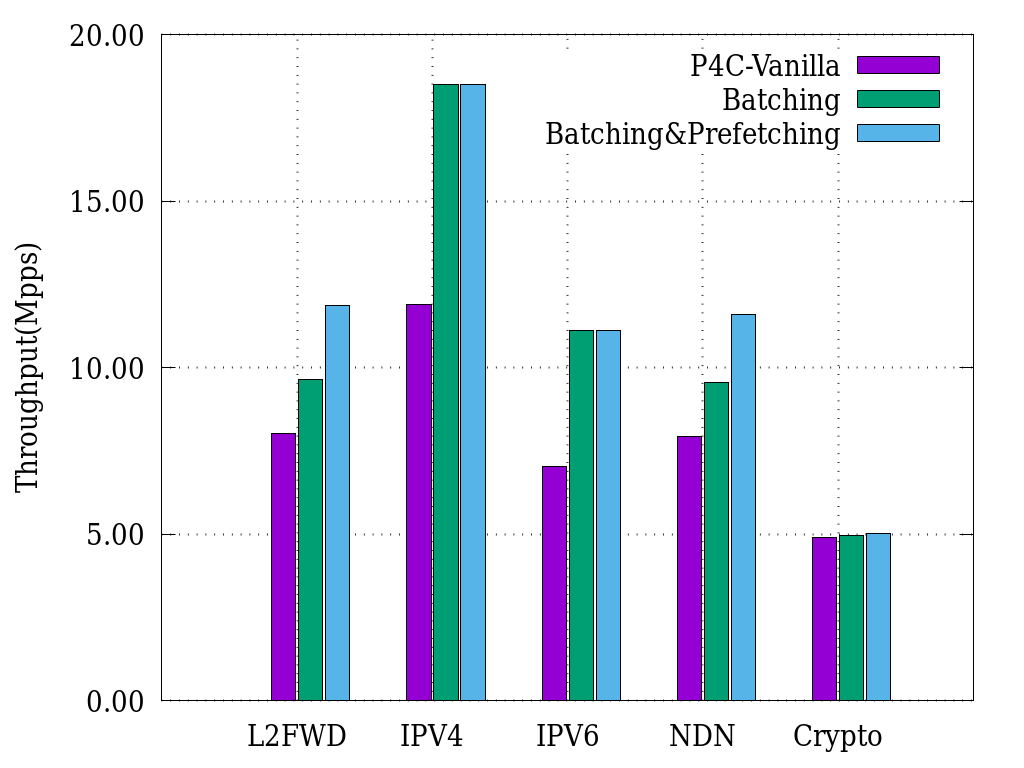
\includegraphics[width = \linewidth]{Figures/effectofbatching.png}
\caption{Effect of batching and prefetching}
\label{fig:batchingandprefetchingfigure}
\end{figure}
We added batching and sub-batching support to P4C, and show results for batch-size $B=32$
in Figure~\ref{fig:batchingandprefetchingfigure}. The {\tt Batching} results represent the case when sub-batching
is disabled (i.e., sub-batch-size $b=1$), while the {\tt Batching and Prefetching} results represent the case
when sub-batching (and prefetching) is enabled and set to its maximum possible value, i.e., sub-batch-size $b=32$.
We later discuss the sensitivity of
throughput to changing $B$ and $b$.
For L2 forwarding, batching improves the performance by 20\% and sub-batching further improves the performance by an additional 23\%. Similarly
for NDN, batching alone improves the performance by 20\% and sub-batching results in an additional performance gain of 21\%.
Using $B=32$ and $b=32$ for IPv4 and IPv6, we obtain a performance gain of 55\% \& 57\% respectively.
For a compute-intensive application like L2Fwd-Crypto, the performance improvements are much smaller.

%In P4C\cite{Laki:2016:HSP:2934872.2959080}, authors are not using batching and prefetching for the applications. We are adding batching and prefetching for all the applications and in Figure \ref{batchingandprefetchingfigure} we are showing the effect of these optimizations for different applications. We are using 32 as batch size for all the applications in all the experiments unless specified otherwise. L2Fwd and NDN are using hash lookup and DPDK code is written in such a way that we are able to prefetch the bucket where the key is present. On the other hand, we don't have much opportunity to use prefetches for LPM lookup based applications. For L2Fwd, batching improves the performance by 20\% and prefetching, used with batching, again improves the performance by 23\%. Similarly for NDN, batching alone improves the performance by 20\% and after adding prefetching there is an additional performance gain of 21 \%. After applying batching and prefetching to IPv4 and IPv6 there is a performance gain of 55\% \& 57\% respectively.
%\\
%\\

%\textbf{Conclusion:} As we can see that batching can be used for almost all the applications without thinking much. However,. Section \ref{optimalbatchsize} can be used to find the optimal batch size. Prefetch on the other hand surely improves the performance but can't be used in every application and should be used with precaution as it might pollute the cache which might result in performance loss.

\subsection{Sensitivity of Throughput to $B$}
We use the L2 forwarding application to demonstrate the effects of changing application behaviour on the optimal
values for $B$ and $b$. We use the L2Fwd application with five different sizes of the lookup table. The size of
the lookup table approximately represents the working set of the application. If the table fits in the caches,
then the application is largely compute bound and has few accesses to the main memory. On the other hand, if the
table is much larger than the last-level cache, then almost every random table access will result in an access to
the main memory. Consequently, the changing application behaviour results in change in the value of the
optimal $B$ and $b$, required for optimal throughput.

Figure~\ref{fig:tablesize} plots the results for throughput for different table sizes and batch-sizes $B$. The solid
line represents the case when the sub-batch-size $b$ equals the batch-size $B$, i.e., $b=B$. The dotted line represents
the case when the sub-batch-size $b=1$, i.e., no sub-batching.

There are a few conclusions to draw from this plot: (1) Expectedly, throughput is generally higher
for smaller tables than for larger tables. (2) For all table sizes, the throughput usually increases with
increasing $B$, due to better exploitation of DMA bandwidth. (3) A batch-size beyond 128, usually results in
decreased throughput due to greater stress on the caching subssystem. (4) Sub-batching improves the throughput
for larger table-sizes, but does not improve throughput for smaller table sizes. This is expected
because sub-batching benefits from memory-level parallelism. For small table-sizes, the main-memory
accesses are few, and so the benefit of sub-batching is little. We discuss this in more detail
in our next experiment. (5) $B=32$ provides near-optimal results across all configurations of the
L2 forwarding application.

\begin{figure}[ht]
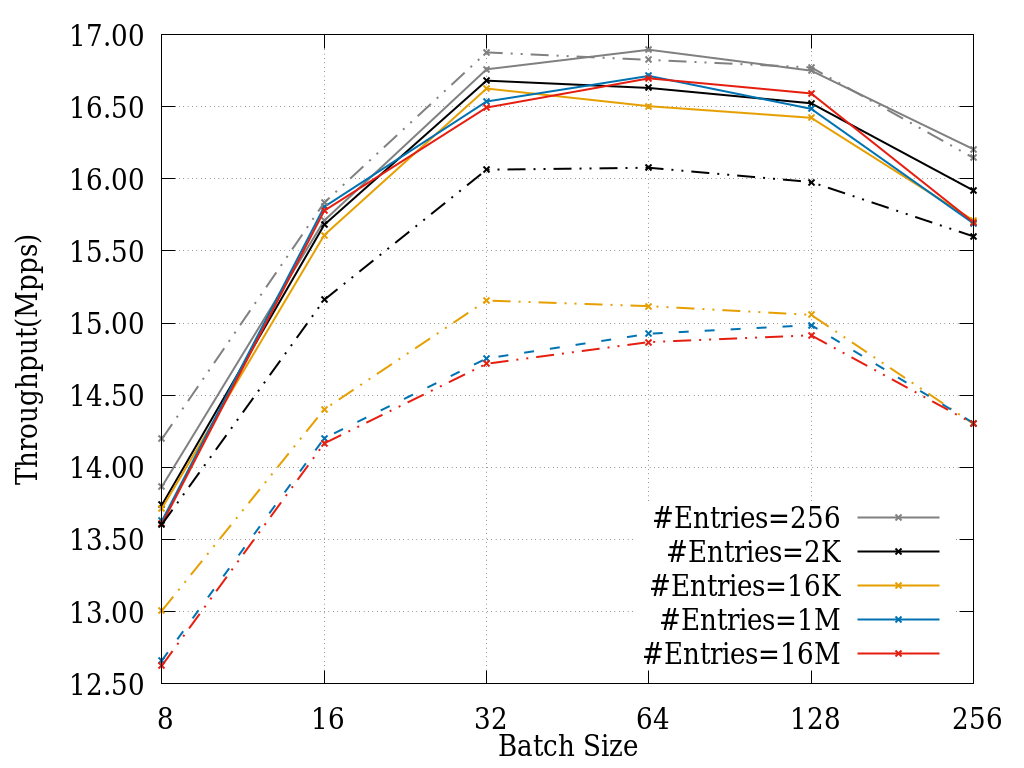
\includegraphics[width = \linewidth]{Figures/TableSizeVsbatchSize.png}
\caption{The effect of batch-size $B$ on application throughput, for five different configurations of the L2 forwarding application. The solid line represents $b=B$ (sub-batching enabled), and the dotted line represents $b=1$ (sub-batching disabled).}
\label{fig:tablesize}
\end{figure}

\begin{figure}[ht]
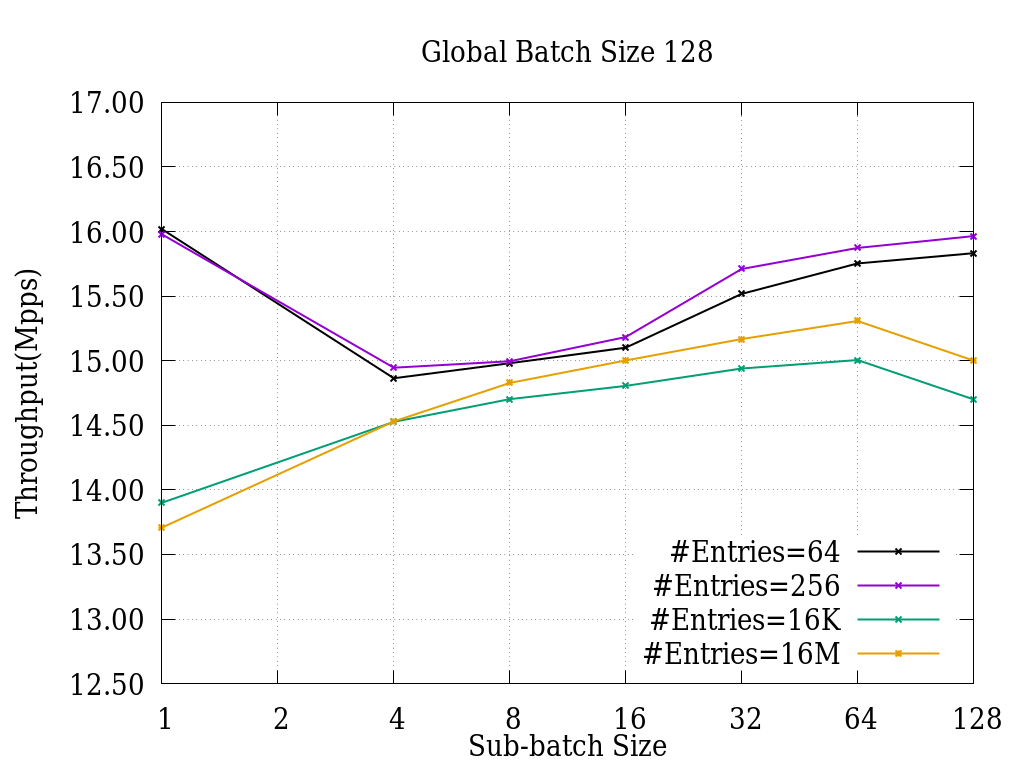
\includegraphics[width = \linewidth]{Figures/Subbatching.png}
\caption{The effect of sub-batch-size $b$ on application throughput, for four different configurations of the L2 forwarding application. We use batch-size $B=32$ for these experiments.}
\label{fig:subbatchfigure}
\end{figure}

\subsection{Sensitivity of Throughput to $b$}

To further understand the sensitivity of application throughput to the sub-batch-size $b$, we vary
$b$ for a fixed value of $B=128$, for the L2Fwd application. Figure~\ref{fig:subbatchfigure} plots
the results, again for different table-sizes. It is interesting to see
that if the table-size is less than, or equal to 256 entries, the throughput
{\em decreases} with increasing batch-size. On the other hand, if the table-size
is large (indicating that many table accesses will be cache misses), the
increasing sub-batch-size, generally improves throughput. If the sub-batch-size
is too large, (e.g., if it is 128 in this case), the performance usually dips
a bit due to increased pressure on the caching subsystem, caused by the
increased memory footprint.

These results confirm that while sub-batching is useful for memory-bound
applications, it is not effective (or sometimes even harmful) for
compute-bound applications. We try and capture this formally in our
performance model, discussed later.

%In Figure \ref{tablesize}, we are showing the relation between throughput and batch size for different number of entries in the lookup table. We are using L2-FWD application with one lookup for this experiment. In the graph, solid lines are representing the results for batching plus prefetching case and dotted lines are representing batching only results. In Section \ref{batchingsubsection} we will talk about the effect of batching on the application with varying number of entries in the table and in Section \ref{prefetchingsubsection} we will take both batching and prefetching into consideration.
%In this experiment we are using IO and Compute batch size 128 and changing the subbatch size to confirm the effect of subbatching. As we can see in the Figure\ref{subbatchfigure} we are able to get improved performance in case of subbatches used in L2Fwd application.
%\subsubsection{Effect of Batching}
%\label{batchingsubsection}
%The throughput is decreasing with increase in the number of entries for the same batch size. This kind of behavior is expected and can be explained with the help of Eq. \ref{compute_througput}. Eq. \ref{compute_througput} and Eq. \ref{cycles_compute} tell that with the help of batching we can amortize per packet cost and the throughput of the application is improved. There is an improvement in the throughput until we are increasing the batch size from 1 to optimal batch size and after that, there is a decline in the throughput.
%\\
%\textbf{Batch Size vs Throughput:} Optimal batch size is different for different cases and can be explained individually for each case. When tables size is small and can fit in L1/L2/L3, the optimal batch size is 32 and if we are increasing the batch size more than 32 then there is a small dip in performance because of the increased cache contention due to increased batch size. However when the table size is bigger than the LLC, for every packet the fetch time is constant and we can increase the batch size to get the benefits of batching. In case of large table size, the optimal batch size is 128 in our case.
%\\
%\textbf{Table Size vs Throughput:} As mentioned in the eq \ref{compute_througput}, memory stall is one of the parameters which is affecting the application throughput. Contention for cache will increase with the increase in the number of entries in the lookup table and this will increase the fetch time for lookup data. So, total fetch time will be more for large table size and less for smaller table size. As explained in Eq \ref{cycles_stall}, we can hide the memory stalling by prefetching the data in the cache. If we can prefetch the data efficiently before the data is used by the application then the total stall time for the batch would decrease and performance of the application would increase.
%
%\subsubsection{Effect of Batching plus Prefetching}
%\label{prefetchingsubsection}
%With prefetching, we are trying to minimize the total stall time for the batch and we can see in the figure that there is a significant performance gain if we are using prefetching with batching. We can summarize the result in two main points. First, there should be a decline in the throughput with the increase in the number of entries and throughput of the application should be more when there are less number of entries in the table. For larger table size, data won't be present in the cache and application must stall on it. However, we are prefetching the data even before the data is used in the application and this prefetching of data is reducing the total stall cycles as described in Eq \ref{cycles_stall}. In case of batching plus prefetching both CPU and memory are working effectively and there are not stall in this case and this is the reason that the throughput of the application is stable and not varying much with the increase in the number of entries in the table.

%Second, for each batch size, the relative throughput of the application will be dictated by the number of entries in the table. In actual, the results are quite opposite to the expectations and this is because total stall time reduction is dependent on effective prefetch distance. One batch size may not work for the different number of entries and relation between table size, batch size, and effective prefetch distance has been summarized in Section \ref{subbatching}. Let's explain with the help of an example, for 64 batch size the throughput of the application is more when there are 1 M and 16 M entries as compared to 2 K \& 16 K entries in the table. The data will be in L2/L3 cache for these many numbers of entries and due to large batch size, entries will be prefetched way before the data will be needed in the application. On the other hand for larger table sizes, larger batch size is suitable since the data will be fetched from the main memory which will take more number of cycles. For 2 K and 16 K entry table we tried to minimize the prefetch distance by using the sub-batch size of 32 and the application is performing better than the application with 1 M and 16 M entries. 
%\textbf{Conclusion:} 
%In case of batching only, the performance is decreasing with an increase in table size because of the increase in the stall time. We are using prefetching to minimize the stall time and in case of batching plus prefetching the throughput is not declining much due to increase in the table size. We can say that batching and prefetching is playing well together and due to this the throughput is stable even if we are increasing the table size.

%\subsection{Sub-batching}
\subsection{Performance model}
We discuss a performance model to explain our experimental results. At a high-level,
the system can be modeled as a queuing network, with three parallel relevant
server components: namely,
the CPU, the CPU-memory interface, and the I/O-memory DMA interface. Assuming that
the three components
can execute in parallel, and have service rates $c$, $m$, and $d$, respectively, the
final throughput of the system would be:
$$
min(c, m, d)
$$
In other words, the throughput of the system is limited by the slowest component (each
packet is expected to traverse all three components).

With batching, we allow multiple in-flight packets on the DMA interface, and
hence increase the parallelism and service rate $d$. If the batch-size is $B$, then
the ideal improvement in the service rate of the DMA interface would be linear ($B*d$).
However, the interface is not fully parallelizable, and so the service rate of
the DMA interface increases as some function $f_{dma}(d, B)$. The plot in Figure~\ref{fig:XXX}
can be used to roughly approximate the shape of this function $f_{dma}$ with increasing value of $B$.

Similarly, with sub-batching, we allow multiple in-flight memory requests on the
CPU-memory interface, and hence increase the service rate $m$. If the batch-size is $b$,
let's assume that the service rate of the CPU-memory interface is denoted by
a function $f_{mem}(m, b)$. The shape of $f_{mem}$ can be roughly approximated using
the plots in Figure~\ref{fig:XXX}. As we can see, the shape of both functions $f_{dma}$
and $f_{mem}$ are dependent on the characteristics of the application. For example,
if the application is compute-bound, $f_{mem}$ typically decreases with increasing $b$.
On the other hand, $f_{mem}$ increases with increasing $b$, for memory-bound applications,
if $b<128$.

Finally, if any improvements can be made to the CPU processing logic (e.g., see discussion
in Section~\ref{sec:discussion}), then those
are counted towards improvements in $c$. In summary, with batching and sub-batching, the
throughput of an application can be represented as:
$$
min(c, f_{dma}(m, b), f_{mem}(d, B))
$$

Thus, a compiler should first estimate the characteristics of the application. For example,
the compiler may run the application for different configurations in an offline
phase, to make conclusions about the degree of compute-boundedness ($c$), memory-boundedness ($m$),
and I/O-boundedness ($d$) of that application. Then, given a machine, the compiler may
use this information with the model
presented above to decide the optimal values for $b$ and $B$.

While our model is preliminary, it does provide an initial basis for reasoning about
performance while generating code for packet processing pipelines.

\subsection{Comparison with other related work}
\label{comparisonexperiment}
\begin{figure}[ht]
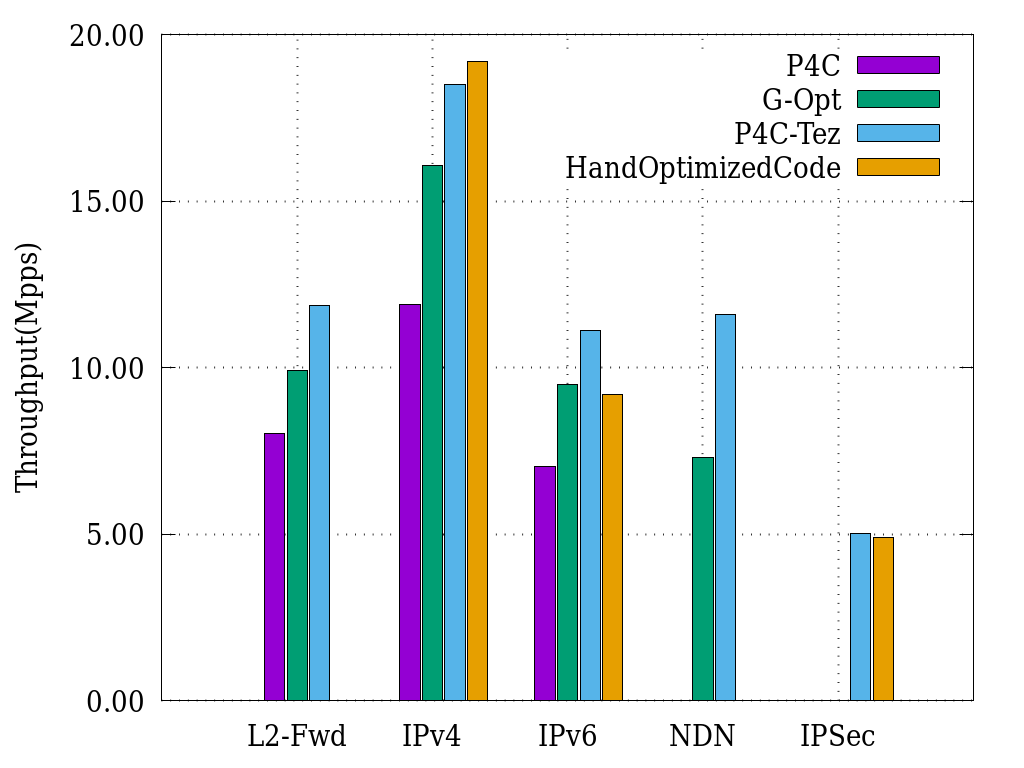
\includegraphics[width = \linewidth]{Figures/comparison.png}
\caption{Comparison with other related work.}
\label{comparisonfigure}
\end{figure}
Figure \ref{comparisonfigure} compares our automatic generated code with vanilla P4C \cite{Laki:2016:HSP:2934872.2959080},
with another
related work, G-Opt, aimed at extracting memory-level parallelism through manual annotations \cite{189006},
and comparable
hand-optimized code available as a part of the DPDK distribution.
To ensure fair comparisons, we verify that the number of lookups and number of entries in the table(s) is same in all experiments.
In cases where a hand-optimized version or GOpt results are not available, we
the corresponding throughput bar is omitted.

Comparing with vanilla P4C, we obtain 48\%, 55\%, 57\%, and 46\% throughput improvements for L2Fwd, IPv4, IPv6, and NDN applications respectively.
The L2Fwd-crypto application shows minimum improvements, due to its inherently compute-intensive nature.
%In the applications, they are not exploiting batching \& prefetching and just with these optimizations there is a huge improvement.
\\
G-Opt is a previous effort at bridging the gap between CPU and GPU performance for packet processing
applications. The G-Opt authors manually annotate code to identify expensive memory accesses, and use
multi-threading and context-switching to hide the memory latency. There are two important ways in which
our work differs from G-Opt: (1) our approach is largely automatic and works with a high-level
program representation. (2) we employ batching and sub-batching instead of multi-threading, which
makes our approach more efficient as it avoids context-switching overheads.
We report a 20\%, 15\%, 17\%, and 59\% improvement over G-Opt for L2Fwd, IPv4, IPv6, and NDN applications respectively,
in head-to-head comparisons. We also find that G-Opt did not systematically explore the space of
all possible transformations, when compared with our work. Our systematic exploration of $B$ and $b$, allows
us to maximize the throughput, beyond previous work.
%They are using both batching and prefetching, and their main aim was to make the results comparable to GPU. The difference is due to the batch size, they are not using the optimal batch size and we can see the performance gain by using the optimal batching size in Figure \ref{tablesize}.
%\\

Comparing with hand-optimized code available as a part of the DPDK distribution, we find that we are sometimes
slightly worse (4\% worse for IPv4), and sometimes significantly better (20\% better for IPv6). It is not
surprising that our compiler-based approach of systematic exploration across the parameter space, can perform
better than hand-optimized code written by developers.
%\textbf{Comparison with DPDK\cite{DPDK}:} For IPv4 DPDK is performing 4\% better than our code and for IPv6 we have a performance gain of 20\%. The result for IPv6 doesn't include the improvement we are gaining by TRIE compression, that will be reported later in this section.
%\\
%\\
%\textbf{Conclusion:} By using the optimal batch size and right prefetch distance we are performing almost equal or better than other hand-tuned optimized code. Even if the results are equal we can say that our approach is better than hand-tuned one, because it is one-time efforts and can be used for wide variety of applications. Results in figure \ref{comparisonfigure} are for one core and we will show in Section \ref{scalability} that our applications are scaling linearly with the number of cores.

\subsection{Scalability}
\label{scalability}
\begin{figure}[ht]
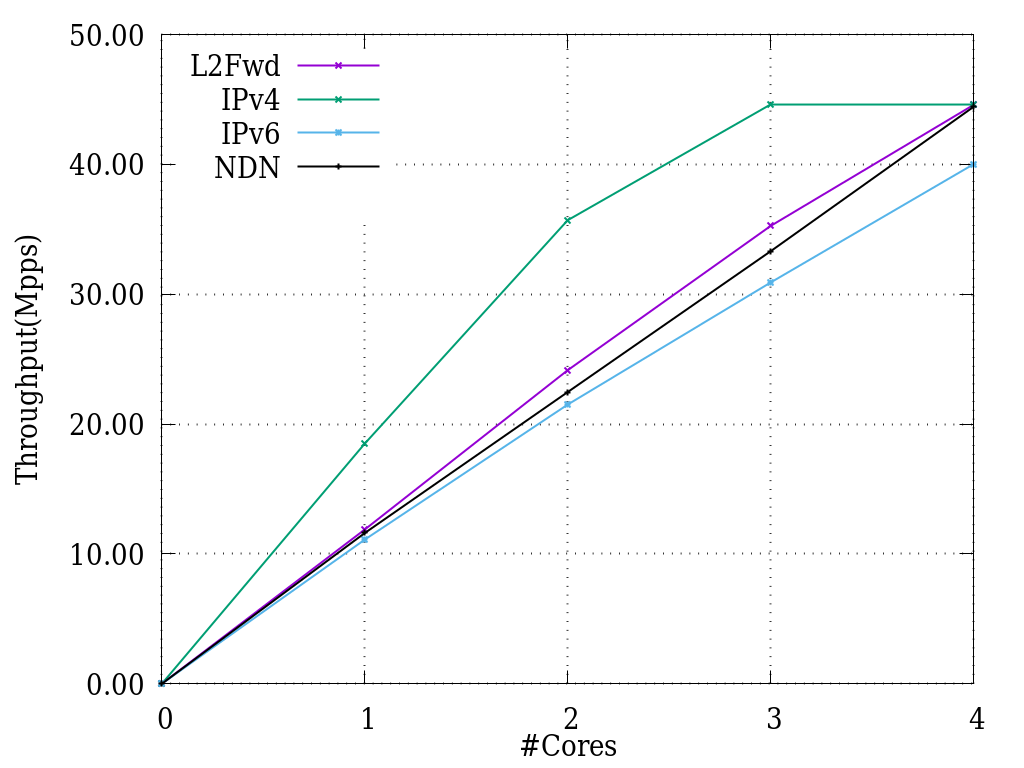
\includegraphics[width = \linewidth]{Figures/cores.png}
\caption{Number of Cores vs Throughput}
\label{cores}
\end{figure}
Figure \ref{cores} plots the application throughput with increasing number of cores.
Unsurprisingly, the throughput usually scales linearly with the number of cores, except when
they saturate the PCIe bandwidth. In our experimental setup, the theoretical max achievable
throughput for 64 byte packets, summed across 4 NICs, is 59 Mpps (million packets per second). However, our
experimental results show that it cannot sustain this theoretical limit, and instead
saturates at 44Mpps. This difference between theoretical and observed throughputs,
is attributed to the fact that the same NICs are being used to both send and
receive packets, resulting in complex scheduling dependencies at the PCIe level.
IPv4 throughput hits the PCIe bandwidth limit in our experimental setup.
IPv6 packet throughput is slightly lower than others, because it uses larger
(78-byte) packets.

%
%With 4 cores we saturating 4 ports(4 x 10 Gbps) when the packet size is 64 bytes.
%The theoretical limit for 4 NICs is 59 Mpps but we are getting 44 Mpps as shown in the graph. PCIe is the bottleneck in this case and not the applications. When one NIC is sending and receiving at both the port then it can reach up 22 Mpps and not theoretical maximum 29 Mpps. \cite{Zhou:2013:SHP:2535372.2535379} has also mentioned about this bottleneck in the paper.

%There is not much to talk about L2Fwd and NDN application, these applications are scaling linearly. IPv6 is not reaching upto 44 Mpps with 4 cores and that is because of large packet size for IPv6. We are using 64 bytes packets for other applications but Pktgen-DPDK is generating 78 bytes packets for IPv6. Hence IPv6 application is also saturating the ports with 4 cores. The other interesting part of the graph is the IPv4 line, till 2 cores the application is scaling linearly and after that it is coming down. There is no more available bandwidth for the application and it is saturating it with three cores. 
%\\
%\textbf{Conclusion:}We can say two things about the result of this experiment. First, applications are scaling linearly with the number of cores and second, applications are saturating four 10 Gbps ports with four cores.


\section{Discussion}
\subsection{TRIE Compression}
In this experiment we enabled the DIR24-8\cite{Gupta98routinglookups} based DPDK LPM6 library to use TRIE compression. The number of steps involved in DIR24-8 based LPM6 matching algorithm is proportional to IPv6 prefix length and in each step, algorithm accesses a new TRIE node which is an expensive memory operation. In real world scenario, IPv6 prefixes can be stored in compressed form in TRIEs either because they are unique or because they have common prefixes. In compression algorithm, we have merged a child node with its parent if it is the only child of its parent.
\\
\textbf{Experiment:} We have populated 20,000 IPv6 prefixes, all having length 48, with varying degree of compression possible.
\\
\textbf{Results:} In the best case, when there were three lookups saving on an average, we have got 38\% higher throughput over DIR24-8 based TRIE and in the worst case, when there is no compression possible, compressed TRIE showed only a dip of 3.3\% in overall throughput. On an average, with 1.25 lookups saving, we got 16.1\% higher throughput than DPDK LPM6 lookup algorithm.



\subsection{Scalability}
\section{Related Work}
\label{relatedwork}
\textbf{CPU based packet processing:} RouteBricks\cite{dobrescu2009routebricks} is one of the first paper in this area. They exploited various components in a commodity server to achieve 35 Gbps throughput for Layer 3 Forwarding. They used both inter-server and intra-server optimizations to achieve this throughput.
\\
\textbf{Manual optimizations:} There are many papers where authors have come up with different kind of manual optimizations to show the improvement in the performance. Batching\cite{dobrescu2009routebricks, 189006, Kim:2012:PBC:2349896.2349910, Zhou:2013:SHP:2535372.2535379} has been used extensively by authors, however, these papers are determining the batch size by empirical analysis. \cite{189006, Zhou:2013:SHP:2535372.2535379} are exploiting the fact that CPU and Memory subsystem can work in parallel and memory stall can be minimized by issuing the software prefetches before actually using the data. However, it is difficult to use these manual optimizations each time we are writing a packet processing application.
\\
\textbf{Compiler optimizations:} Shangri-La \cite{Chen:2005:SAH:1065010.1065038} generates optimized binary for network processor and showing that the generated binary is working as good as hand-tuned code. \cite{Dobrescu:2010:CPM:1921151.1921154} talks about the importance of doing the optimizations in the compiler rather than hand-tuning the same thing for different applications. The main focus of paper \cite{Dobrescu:2010:CPM:1921151.1921154} is to automating the decision of breaking the application in parallel components to achieve high throughput.
Due to space constraint, we are not mentioning papers related to various kind of software based packet processors and different DSLs for writing the network applications.

In our L2 forwarding example, there are two table lookups, both of which can potentially result
in main-memory access (and CPU stalls). Indeed the CPU stalls only occur if the lookup table
cannot fit in memory {\em and} the entry being looked-up is not already present in the cache.
Both these criteria are impossible to judge statically, and an automatic compiler-based
approach enables online dynamic code regeneration to adapt to the workload needs.



\section{Conclusion}
\label{section6} 
The goal of this paper is to find the efficient batch size and right prefetch distance to use the underlying hardware efficiently and to improve the application performance. In the evaluation section, we are showing that per core performance for different applications is on par with hand-tuned optimized applications and applications are scaling with the number of cores. It saves a lot of time and efforts, and we don't need to think about the code flow for different types of applications and the possible bugs due to manual intervention. We believe that DSLs won't be very useful if we are unable to develop good compilers. The actual power of DSLs can only be realized when the compilers can generate the optimized target which is on par with hand-tuned code.
